\documentclass[11pt]{article}

\usepackage[french]{babel}

\usepackage[utf8]{inputenc}
\usepackage{palatino}
\usepackage[T1]{fontenc}


\usepackage{url}
\usepackage{amsmath}

\usepackage[top=2cm,bottom=2cm,left=2.1cm,right=2.1cm,headsep=10pt,a4paper]{geometry}
\usepackage{fancyhdr}


\usepackage{graphicx,float,subcaption} % figure et placement de figure

\pagestyle{fancy}
\lhead{}
\chead{\fontsize{10}{10}{LIP - 2018}}
\rhead{\thepage}
\lfoot{\fontsize{10}{10}{Rapport de stage}}

\renewcommand{\headrulewidth}{0pt}
\renewcommand{\footrulewidth}{0pt}



 \author{\fontsize{14}{14}{\bf Arthur Gontier}\\
\fontsize{14}{14}{Encadrement: Laure Gonnord}}
\title{\fontsize{16}{16}{{\bf Rapport}}}

      
\date{\fontsize{11}{11}{2018}}

\usepackage[T1]{fontenc}
\usepackage{graphicx}
\usepackage{grffile}
\usepackage{longtable}
\usepackage{wrapfig}
\usepackage{rotating}
\usepackage[normalem]{ulem}
\usepackage{amsmath}
\usepackage{textcomp}
\usepackage{amssymb}
\usepackage{capt-of}
\usepackage{hyperref}% \documentclass[a4paper,11pt]{article}
% \usepackage[margin=2cm]{geometry}
% \usepackage[utf8]{inputenc}

\usepackage{graphicx} 
\usepackage{wrapfig}
\usepackage{color}
\usepackage{xcolor}
\usepackage{hyperref}



\usepackage[]{amsmath,amsfonts,amssymb,stmaryrd,amsthm}
\usepackage{fullpage}
\usepackage{multirow}
\usepackage[rounded]{syntax}
\usepackage[section]{placeins}
\newtheorem{example}{Exemple} %%% modifier ici si on veut en fr/en

\usepackage{todonotes}

%\input{macros}

\usepackage{listings} 


\usepackage{listings}
\usepackage{inconsolata} % very nice fixed-width font included with texlive-full
%\usepackage[usenames,dvipsnames]{color} % more flexible names for syntax highlighting colors

\definecolor{chameleond}{HTML}{4E9A06}
\definecolor{skyblued}{HTML}{204A87}
\definecolor{darkgreen}{HTML}{006400}

%\usepackage[usenames,dvipsnames]{color} % more flexible names for syntax highlighting colors


\lstset{
basicstyle=\ttfamily, 
columns=fullflexible, % make sure to use fixed-width font, CM typewriter is NOT fixed width
numbers=left, 
numberstyle=\small\ttfamily\color{gray},
stepnumber=1,              
numbersep=10pt, 
numberfirstline=true, 
numberblanklines=true, 
tabsize=4,
lineskip=-1.5pt,
extendedchars=true,
breaklines=true,        
keywordstyle=\color{skyblued}\bfseries,
identifierstyle=, % using emph or index keywords
commentstyle=\sffamily\color{darkgreen},
stringstyle=\color{chameleond},
showstringspaces=false,
showtabs=false,
upquote=false,
texcl=true % interpet comments as LaTeX
}


\lstset{literate=
  {α}{{$\alpha$}}1 {Δ}{{$\Delta$}}1
  {á}{{\'a}}1 {é}{{\'e}}1 {í}{{\'i}}1 {ó}{{\'o}}1 {ú}{{\'u}}1
  {Á}{{\'A}}1 {É}{{\'E}}1 {Í}{{\'I}}1 {Ó}{{\'O}}1 {Ú}{{\'U}}1
  {à}{{\`a}}1 {è}{{\`e}}1 {ì}{{\`i}}1 {ò}{{\`o}}1 {ù}{{\`u}}1
  {À}{{\`A}}1 {È}{{\'E}}1 {Ì}{{\`I}}1 {Ò}{{\`O}}1 {Ù}{{\`U}}1
  {ä}{{\"a}}1 {ë}{{\"e}}1 {ï}{{\"i}}1 {ö}{{\"o}}1 {ü}{{\"u}}1
  {Ä}{{\"A}}1 {Ë}{{\"E}}1 {Ï}{{\"I}}1 {Ö}{{\"O}}1 {Ü}{{\"U}}1
  {â}{{\^a}}1 {ê}{{\^e}}1 {î}{{\^i}}1 {ô}{{\^o}}1 {û}{{\^u}}1
  {Â}{{\^A}}1 {Ê}{{\^E}}1 {Î}{{\^I}}1 {Ô}{{\^O}}1 {Û}{{\^U}}1
  {œ}{{\oe}}1 {Œ}{{\OE}}1 {æ}{{\ae}}1 {Æ}{{\AE}}1 {ß}{{\ss}}1
  {ű}{{\H{u}}}1 {Ű}{{\H{U}}}1 {ő}{{\H{o}}}1 {Ő}{{\H{O}}}1
  {ç}{{\c c}}1 {Ç}{{\c C}}1 {ø}{{\o}}1 {å}{{\r a}}1 {Å}{{\r A}}1
  {€}{{\EUR}}1 {£}{{\pounds}}1
}

% \lstset{language=bash,
% stringstyle=\ttfamily,
% basicstyle=\footnotesize, 
% showstringspaces=false,
% breaklines=true,
% }

\lstdefinestyle{numbers} {numbers=left, stepnumber=5, numberstyle=\tiny, numbersep=10pt}
% \lstdefinestyle{lc3} {language=[x86masm]Assembler,style=numbers,frame=lines,showstringspaces=false,keywords={BR,LD,BRz,BRn,BRzp,BRnz,BRnzp,LEA,HALT,RET,.END,.ORIG,.FILL,.STRINGZ,PUTS,ADD,AND,OR,OUT,NOT,LDR,STR,JSR,NOP,GETC},showstringspaces=false,keepspaces=true,flexiblecolumns=true,deletekeywords={end}}

\lstdefinestyle{target}
{language=[x86masm]Assembler,style=numbers,frame=lines,showstringspaces=false,keywords={add,
  jump, snif,call,return,.string,.reserve,.word,.set,.align16,letl,leth,.let,and,or,wmem,rmem,asr,xor,sub,sgt,sle,slt,slt},showstringspaces=false,keepspaces=true,flexiblecolumns=true,deletekeywords={end},breaklines=true}



%\definecolor{chameleond}{HTML}{4E9A06}
%\definecolor{skyblued}{HTML}{204A87}


\lstdefinestyle{digmips} {language=[x86masm]Assembler,style=numbers,frame=lines,showstringspaces=false,keywords={add,sub,ld,ldi,ble,j,jmp,st},showstringspaces=false,keepspaces=true,flexiblecolumns=true,deletekeywords={end},keywordstyle=\color{skyblued},commentstyle=\color{red}\bf,morecomment=[l][\color{red}]{//}}


\lstdefinestyle{lc3} {language=[x86masm]Assembler,style=numbers,frame=lines,showstringspaces=false,keywords={BR,LD,BRz,BRn,BRzp,BRnz,BRnzp,LEA,HALT,RET,.END,.ORIG,.FILL,.STRINGZ,PUTS,ADD,AND,OR,OUT,NOT,LDR,STR,JSR,NOP,GETC},showstringspaces=false,keepspaces=true,flexiblecolumns=true,deletekeywords={end}}


\lstdefinelanguage{[Objective]Caml}
{basicstyle=\ttfamily,
keywordstyle=\itshape\bfseries,
identifierstyle=,
stringstyle=\itshape,
commentstyle=\itshape,
flexiblecolumns=true,
escapechar=\%}

\lstdefinelanguage{julia}
{
  keywordsprefix=\@,
  morekeywords={
    exit,whos,edit,load,is,isa,isequal,typeof,tuple,ntuple,uid,hash,finalizer,convert,promote,
    subtype,typemin,typemax,realmin,realmax,sizeof,eps,promote_type,method_exists,applicable,
    invoke,dlopen,dlsym,system,error,throw,assert,new,Inf,Nan,pi,im,begin,while,for,in,return,
    break,continue,macro,quote,let,if,elseif,else,try,catch,end,bitstype,ccall,do,using,module,
    import,export,importall,baremodule,immutable,local,global,const,Bool,Int,Int8,Int16,Int32,
    Int64,Uint,Uint8,Uint16,Uint32,Uint64,Float32,Float64,Complex64,Complex128,Any,Nothing,None,
    function,type,typealias,abstract
  },
  sensitive=true,
  morecomment=[l]{\#},
%  morecomment=[s]{# =}{=#},
  morestring=[b]',
  morestring=[b]" 
}

\lstdefinelanguage{cplus}
{
        frame=lines,
	language=C++,
	basicstyle=\tt,
        morecomment=[l][\color{magenta}]{\#},
	keywordstyle=\color{chameleond},
	identifierstyle=\color{black},
        stringstyle=\color{skyblued},
        commentstyle=\color{red},
	tabsize=4,
}


\lstdefinelanguage{mypython}
{
%        frame=lines,
	language=Python,
	basicstyle=\tt,
        morecomment=[l][\color{magenta}]{\#},
	keywordstyle=\color{chameleond},
	identifierstyle=\color{black},
        stringstyle=\color{skyblued},
        commentstyle=\color{red},
	tabsize=4,
        breaklines=true,
}


\lstdefinelanguage{flexbison}
{
        frame=lines,
	language=C,
	basicstyle=\tt,
        keywords={yylex,yyparse,yyline,yytext,yyin},
        morecomment=[l][\color{magenta}]{\#,},
	keywordstyle=\color{chameleond},
	identifierstyle=\color{black},
        stringstyle=\color{skyblued},
        commentstyle=\color{red},
	tabsize=4,
}


\lstdefinelanguage{antlr}
{
%  frame=lines,
  language=Java,
  basicstyle=\tt\scriptsize,
  breaklines=true,%                                      allow line breaks
  moredelim=[s][\color{blue!50!black}\ttfamily]{'}{'},% single quotes in green
  moredelim=*[s][\color{black}\ttfamily]{options}{\}},%  options in black (until trailing })
  commentstyle={\color{gray}\itshape},%                  gray italics for comments
  morecomment=[l]{//},%                                  define // comment
  emph={%
    STRING%                                            literal strings listed here
  },emphstyle={\color{blue}\ttfamily},%              and formatted in
                                %              blue
  keywords={grammar,header,members,skip},
  alsoletter={:,|,;},%
  morekeywords={:,|,;},%                                 define the special characters
  keywordstyle={\color{chameleond}},%                         and format them in black
}


\lstdefinelanguage{mycaml}
{       language=Caml,
        upquote=true,
        columns=flexible,
        keepspaces=true,
        breakindent=0pt,
        basicstyle=\ttfamily,
        breaklines=true,
        keywordstyle=\color{red},
        commentstyle=\color{darkgreen},
        tabsize=2,
        escapechar=\%,
        escapebegin=\color{blue}
        }

\lstdefinelanguage{myhaskell}
{       language=Haskell,
        upquote=true,
        columns=flexible,
        keepspaces=true,
        breakindent=0pt,
        basicstyle=\ttfamily\scriptsize,
        breaklines=true,
        keywordstyle=\color{red},
        commentstyle=\color{darkgreen},
        tabsize=2,
        escapeinside={!}{!},
        escapebegin=!\endgraf\color{gray},
        }



\newcommand\ocamli[1]{\lstinline[language=mycaml,basicstyle=\ttfamily\normalsize]{#1}}
\newcommand\llvminline[1]{\lstinline[language=LLVM,basicstyle=\ttfamily\normalsize]{#1}}
\newcommand\llvmfile[1]{\lstinputlisting[language=LLVM]{#1}}

\lstnewenvironment{llvmc}{
  \lstset{language=llvm,mathescape,
    basicstyle=\ttfamily\small,
    aboveskip={0\baselineskip},
    belowskip=0\baselineskip
  }}{}


\lstdefinelanguage{lustre}
{
  basewidth={0.5em,0.5em},
  % list of keywords
  morekeywords={
    pre,
    fby,
    ->,
    current,
    when,
    node, 
    returns,
    let,
    tel,
    var,
    if,
    then,
    int,
    bool,
  },
  sensitive=false, % keywords are not case-sensitive
  escapeinside={!}{!},          % if you want to add LaTeX within your code
  morecomment=[l]{//}, % l is for line comment
  morecomment=[s]{/*}{*/}, % s is for start and end delimiter
  morestring=[b]", % defines that strings are enclosed in double quotes
  basicstyle=\ttfamily,
  keywordstyle=\bfseries\color{blue!80!black},
  keywordstyle=[2]\bfseries\color{red!50!white},
  commentstyle=\itshape\color{purple!40!black},
  %identifierstyle=\color{blue!80!black},
  stringstyle=\color{orange}
}


\lstset{language=lustre}

\newcommand{\laure}[1]{\textcolor{red}{#1}}
\newcommand{\arthur}[1]{\textcolor{violet}{#1}}
\newcommand{\lustre}{\xspace{\sc Lustre}\xspace}
\newcommand{\lic}{\xspace{\sc Lic}\xspace}
\newcommand{\smt}{\xspace{\sc SMT}\xspace}

\setcounter{tocdepth}{2}     % Dans la table des matieres
\setcounter{secnumdepth}{3}  % Avec un numero.

\begin{document}

\thispagestyle{empty}
\maketitle



\begin{abstract}

  Rapport

\medskip
  Dans ce travail, nous proposons \arthur{patate} \todo{de trucs}

  Dans ce rapport nous présentons 

\end{abstract}

\tableofcontents

\newpage

\section{exemple julia}

\lstset{language=julia}

{
\begin{lstlisting}
# --------------------------------------------------------------------------- 
  #Loading an instance of SPP (format: OR-library)

function loadSPP(fname)
    f=open(fname)
    # Lecture du nbre de contraintes (m) et de variables (n)
    m, n = parse.(Int, split(readline(f)) )
    # Lecture des n coefficients de la fonction economique et cree le vecteur d'entiers C
    C = parse.(Int, split(readline(f)) )
    # Lecture des m contraintes et reconstruction de la matrice binaire A
    A=zeros(Int, m, n)
    for i=1:m
        # Lecture du nombre d'elements non nuls sur la contrainte i (non utilise)
        readline(f)
        # Lecture des indices des elements non nuls sur la contrainte i
        for valeur in split(readline(f))
          j = parse(Int, valeur)
          A[i,j]=1
        end
    end
    close(f)
    return C, A
end

# --------------------------------------------------------------------------- 
# Construction gloutonne d'une solution admissible de SPP

function GreedyConstruction(C_in, A_in)

   # A completer...
   
    return x, z
end

# --------------------------------------------------------------------------- 
# Amelioration gloutonne par recherche locale d’une solution de SPP

function GreedyAmelioration(C_in, A_in, x_in, z_in)

   # A completer...
   
    return xbest, zbest
end

# --------------------------------------------------------------------------- 
# Exemple (compliant Julia v0.7 et ulterieur)

using Printf
fname = "Desktop/Data/pb_200rnd0100.dat"

C, A = loadSPP(fname)

@time x, z = GreedyConstruction(C, A)
@printf("z(xInit) = %d \n\n",z)

@time xbest, zbest = GreedyAmelioration(C, A, x, z)
@printf("z(xBest) = %d \n\n",zbest)
\end{lstlisting}
}
%
% =================================================================================
%
\section{Exemple d'exécution}

\begin{verbatim}
  0.299466 seconds (1.97 M allocations: 532.954 MiB, 11.09% gc time)
z(xInit) = 351 

  0.020743 seconds (9.12 k allocations: 70.348 MiB, 19.62% gc time)
z(xBest) = 357 
\end{verbatim}

\section{exemple d'importation de fichier jl}

\lstset{language=julia}

\begin{figure}
  \centering
  \lstinputlisting{code/RO-l3.jl}
  \caption{Projet de l'an dernier}
  \label{fig:ro-l3}
\end{figure}


\section{Contexte: les langages synchrones et \lustre, les clauses de Horn}
\label{section:background}

\subsection{Le langage \lustre}


\emph{Cette section sur \lustre est inspirée de la documentation de
  \lustre~\cite{LustreRefMan,TutorialLustre} et du rapport
  de stage de Szabolcs-Marton Bagoly~\cite{rapportstagesobi}. }
%rappels sur lustre inspirés du machin en anglais dans les anciennes versions.

\paragraph{blablabla...}
\medskip

\subsection{Nouvelle traduction de l'opérateur \texttt{Mapred/fillred}}

Le fillred est la contraction du red et du fill donc on reprend exactement la même
structure que le fill à laquelle on ajoute des tableaux en entrée. On
illustre ici pour \texttt{(res,x,y) = fillred<<test,4>>(init,a,b)}.

Comme le red, on a pour chaque variable init à gauche, un accumulateur généré
et les trois clauses suivantes :

\begin{center} $t \geq 0 \wedge State_{init}(init,a,b,res,x,y,i,t+1)
  \wedge State_a(init,a,b,res,x,y,0,t+1)\wedge State_b(init,res,x,y,a,b,0,t+1)
  \wedge Interface_{test}(init,a[0],b[0],acc[0],x[0],y[0],t+1) $

  $\implies State_{acc}(init,a,b,res,x,y,0,t)  $
\end{center}

\begin{center} $t \geq 0 \wedge State_{acc}(init,a,b,res,x,y,i-1,t)
  \wedge i > 0 \wedge i<size
  \wedge State_a(init,a,b,res,x,y,i,t+1)\wedge State_b(init,a,b,res,x,y,i,t+1)
  \wedge Interface_{test}(acc[i-1],a[i],b[i],acc[i],x[i],y[i],t+1) $

   $\implies State_{acc}(init,a,b,res,x,y,i,t) $
\end{center}

\begin{center} $t \geq 0 \wedge State_{acc}(init,a,b,res,x,y,size-1,t)
  \implies State_{res}(init,a,b,res,x,y,i,t+1) \wedge res[t] = acc[size-1][t] $
\end{center}

Avec ceci, nous avons calculé les (valeurs des cases des) tableaux mais nous ne les avons pas rendu accessibles.
Pour y remédier, on ajoute la clause suivante pour chaque tableau~:

$t \geq 0 \wedge State_{res}(init,a,b,res,x,y,i,t+1)
\implies State_x(init,a,b,res,x,y,i,t+1) $

(et idem avec $State_{y}(init,a,b,res,x,y,i,t)$)


 \begin{figure}[t!]
    \begin{subfigure}[t]{0.25\textwidth}
  \centering
  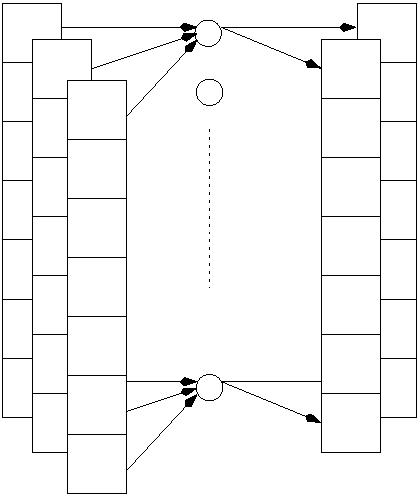
\includegraphics[scale=0.45]{fig/map.pdf}
  \caption{map}
  \label{fig:map}
    \end{subfigure}%
    ~ 
    \begin{subfigure}[t]{0.22\textwidth}
  \centering
  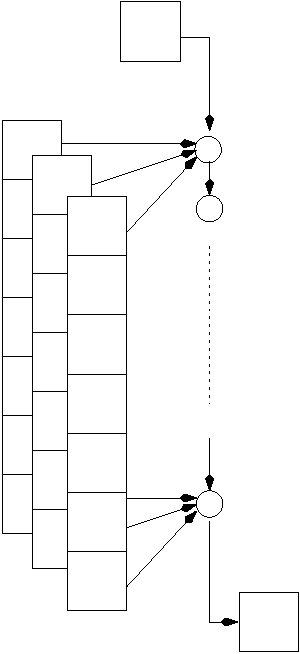
\includegraphics[scale=0.45]{fig/red.pdf}
  \caption{red}
  \label{fig:red}
\end{subfigure}
\begin{subfigure}[t]{0.25\textwidth}
  \centering
  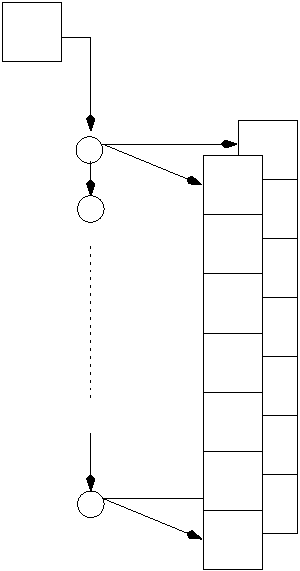
\includegraphics[scale=0.45]{fig/fill.pdf}
  \caption{fill}
  \label{fig:fill}
\end{subfigure}
\begin{subfigure}[t]{0.25\textwidth}
  \centering
  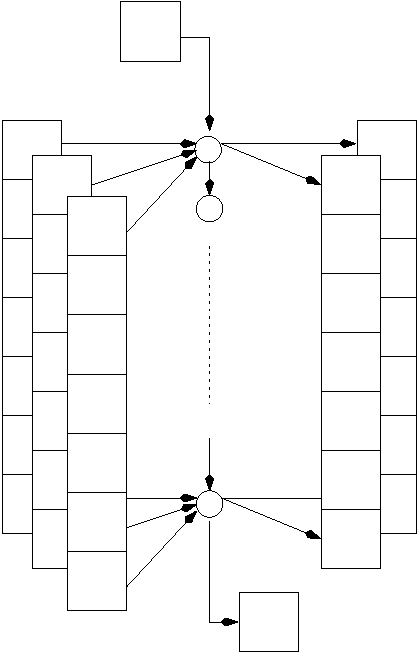
\includegraphics[scale=0.45]{fig/mapred.pdf}
  \caption{fillred}
  \label{fig:fillred}
\end{subfigure}

\caption{Illustration du comportement des itérateurs de tableaux}
\end{figure}

\paragraph{Bugs inexpliqués}
\begin{itemize}
\item unsat quand un map et un red se suivent (sat-det-max, sat-red-pos)
\item sat-bounded-interval ne termine pas
\item le fill sur un tuple non plus
\item et aucun fillred (possibilité d'une erreur dans la traduction)
\end{itemize}

\section{Conclusion}
\label{section:conclusion}

Ce travail porte donc sur

\newpage
\bibliographystyle{plain}
\bibliography{lustohorn}



\end{document}

%%% Local Variables:
%%% mode: latex
%%% TeX-master: "rapport_gontier."
%%% End:
